\section{Results}\label{Sec:Results}

\begin{itemize}

\item Organize material and present results.

\item Use tables, figures (but prefer visual presentation):
\begin{itemize}
\item Tables and figures should supplement (and not duplicate) the
text.

\item Tables and figures should be provided with
legends.\\
{\it Figure \ref{Fig:Resids} shows how to include and reference
graphics. The graphic must be labelled before. Files must be in
\texttt{.eps} format.}

\begin{figure}[ht]
\begin{center}
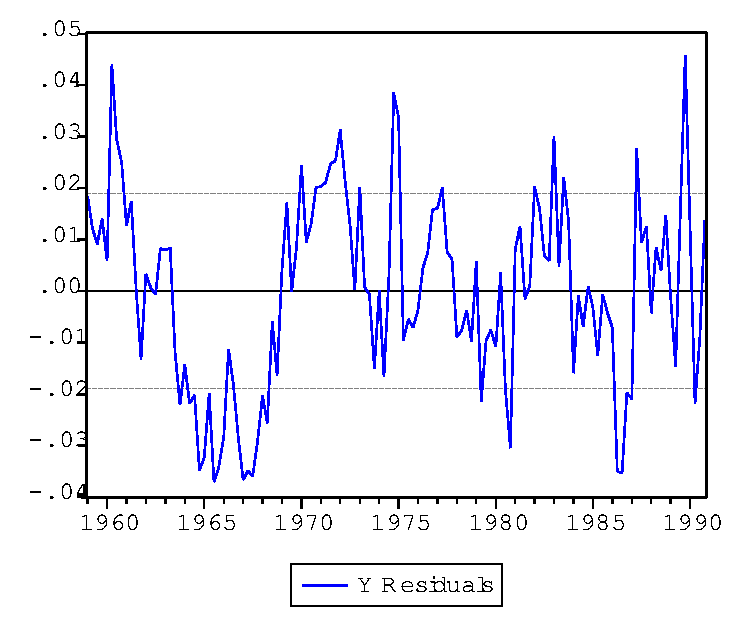
\includegraphics[scale=0.5,angle=0]{graph}
\caption{Estimated residuals from model XXX. ...}
\label{Fig:Resids}
\end{center}
\end{figure}

\item Tables and graphics may appear in the text or in
the appendix, especially if there are many simulation results
tabulated, but is also depends on the study and number of tables resp.
figures. The key graphs and tables must appear in
the text!
\end{itemize}

\item Latex is really good at rendering formulas:\\
{\it Equation (\ref{Eq:SpecDens}) represents the ACs of a stationary
stochastic process:
\begin{equation}
f_y(\lambda) = (2\pi)^{-1} \sum_{j=-\infty}^{\infty}
\gamma_j e^{-i\lambda j}
=(2\pi)^{-1}\left(\gamma_0 + 2 \sum_{j=1}^{\infty}
\gamma_j \cos(\lambda j)\right)
            \label{Eq:SpecDens}
\end{equation}
where $i=\sqrt{-1}$ is the imaginary unit, $\lambda \in [-\pi,
\pi]$ is the frequency and the $\gamma_j$ are the autocovariances
of $y_t$.}

\newpage

\item Discuss results:
\begin{itemize}
\item Do the results support or do they contradict economic theory ?
\item What does the reader learn from the results?
\item Try to give an intuition for your results.
\item Provide robustness checks.
\item Compare to previous research.
\end{itemize}
\end{itemize}

\subsection{Sample Preparation}
FFPE <-> library concentration

Pictures of Bioanalyzer

\begin{figure}[!tbp]
  \centering
  \subfloat[Overlayed Electropherograms of Four Representative Libraries Prepared with Agilent Haloplex CSC]{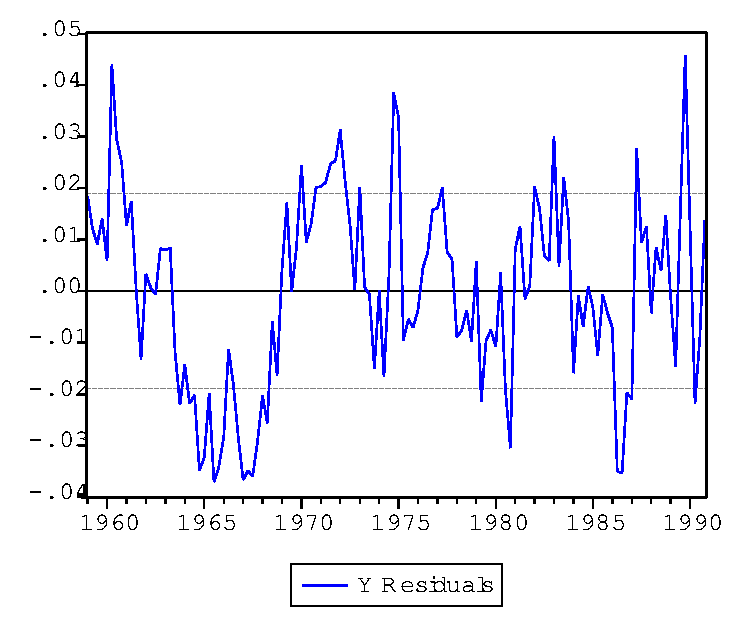
\includegraphics[width=0.45\textwidth]{graph.pdf}\label{fig:f1}}
  \hfill
  \subfloat[Overlayed Electropherograms of Four Representative Libraries Prepared with Illumina TST15 (MixA \& MixB)]{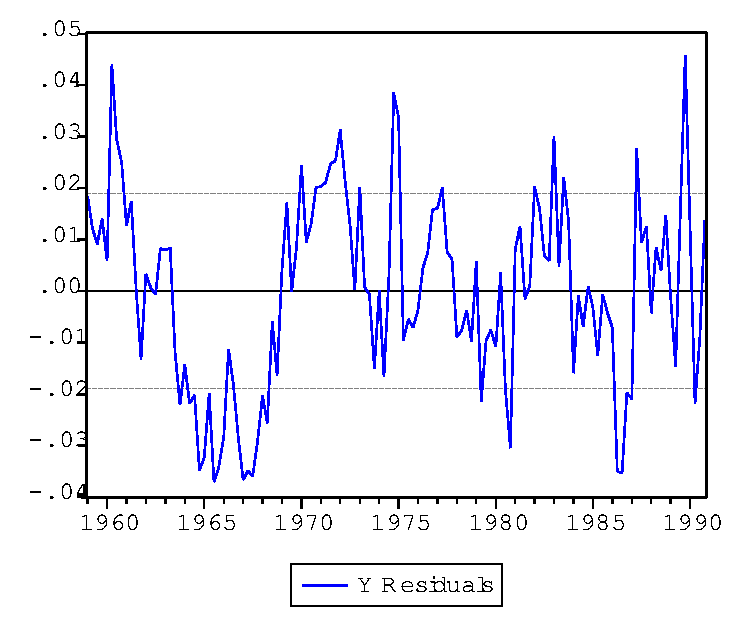
\includegraphics[width=0.45\textwidth]{graph.pdf}\label{fig:f2}}
  \caption{Comparison of Agilent Bioanalyzer Electropherograms}
\end{figure}

\subsection{NGS Data Quality}

Illumina Sequencing Viewer

\begin{table}[!htbp]
    \caption[ISV]{Comparison of Run Parameters (Averaged) of Sequencing Runs with Haloplex CSC \& TST15 Sample Preparation}
    \centering
    \begin{tabular}{ |p{4cm}||p{4cm}||p{4cm}|}
    \hline
    Parameter & Haloplex CSC & TST15 \\ \hline \hline
    Yield total (Gb) & 3.7 & 7.37 \\ \hline
    \% \textgreater Q30 & 93.8 & 82.355 \\ \hline
    Cluster Density PF (k/mm2) & 1084 & 1180  \\ \hline
    Cluster Density PF (%) & 85.95 & 79.95  \\ \hline
  \end{tabular}
\end{table}

FASTQC

Samtools flagstat

{\lipsum[2]

\begin{minipage}{0.5\textwidth}
Blabla bla bla bla cfgvhbjknlmdsc
dc
sdcdscedsvdsv
sdvxsdxyjcnmxceds ecdnc edckcesa sma
\end{minipage}
\hfill
\begin{minipage}{0.5\textwidth}
\captionof{table}{Your caption here}
\begin{tabular}{p{3cm} p{1.5cm} p{1.5cm}}\\
\hline
Parameter & Haloplex CSC & TST15 \\
\hline
\% mapped & 91 & 62.6 \\
\% paired & 0 & 58.7 \\
\% singletons & 1.8 & 3.8 \\
\label{samtools flagstat}
\end{tabular}
\end{minipage}


{\lipsum[2]

GATK ReadLengthDistribution

GATK FlagStat???

\subsection{Coverage Analysis}

Coverage Distribution TST15 vs Haloplex (absolute & normalized to compare if one of them has a larger IQR)

Coverage Distribution per Patient (check if correlation IQR with dCt)

Coverage Distribution per Amplicon (check if some have always lower coverage, check if some failed)
(GATK CallableLoci)
(GATK CountLoci???)
(GATK FindCoveredIntervals)

Failed Amplicon Counter

On-off target; Enrichment Efficiency TST15 vs Haloplex

Coverage across genome, check where there is coverage

Strandedness?

GATK DepthOfCoverage???
GATK FlagStat???
Fragmentation <-> Coverage?


\subsection{Variant Calling Algorithm Comparison}
Detection of Known Single Nucleotide Variants and Deletions

Which should be found?

Which have not been found? Why?

MuTect

VarScan

GATK HaplotypeCaller

SomVarIUS????????
Freebayes????????
Vardict???????

SureCall & TST15

GATK SelectVariants
GATK VariantFiltration
GATK VariantEval
GATK ValidateVariants

More C>T ?
